% coding:utf-8

%----------------------------------------
%FOSAPHY, a LaTeX-Code for a summary of basic physics
%Copyright (C) 2013, Mario Felder

%This program is free software; you can redistribute it and/or
%modify it under the terms of the GNU General Public License
%as published by the Free Software Foundation; either version 2
%of the License, or (at your option) any later version.

%This program is distributed in the hope that it will be useful,
%but WITHOUT ANY WARRANTY; without even the implied warranty of
%MERCHANTABILITY or FITNESS FOR A PARTICULAR PURPOSE.  See the
%GNU General Public License for more details.
%----------------------------------------

\chapter{Bewegung}

\section{Gerade Bewegung}
Die gerade Bewegung kennt vier elementare Grössen: 
Weg $\vec{s}$, Geschwindigkeit $\vec{v}$, Beschleunigung $\vec{a}$ und
die Zeit $t$. Alle diese Grössen, mit Ausnahme der Zeit $t$, sind 
vektorielle Grössen.

Diese drei vektoriellen Grössen, welche alle Funktionen der Zeit
sind, können gegenseiten jeweils durch differenzieren oder integrieren 
nach der Zeit $t$ hergeleitet werden, denn es gilt der folgende 
Zusammenhang.

\[ \boxed{\begin{array}{c c c c c}
	\vec{x}(t) 
		& \xrightarrow{\frac{d}{dt}}
	& \vec{v}(t)
		& \xrightarrow{\frac{d}{dt}}
	& \vec{a}(t) \\
	& & & & \\
	\vec{x}(t) 
		& \xleftarrow{\int dt}
	& \vec{v}(t)
		& \xleftarrow{\int dt}
	& \vec{a}(t) \\
\end{array}} \]

\noindent
Die Definitionen für die Momentanwerte sind dabei die Folgenden.
\[\boxed{\begin{array}{r l}
	\vec{v}	&
		= \displaystyle \lim\limits_{P_2 \rightarrow P_1} 
			{\left( \frac{x_2 - x_1}{t_2 - t_1} \right)}
		= \displaystyle \lim\limits_{\Delta t \rightarrow 0}
			{\frac{\Delta x}{\Delta t}}
		= \displaystyle \frac{\mathrm{d}x}{\mathrm{d}t}=\dot{x} \\
	& \\
	\vec{a} &
		= \displaystyle \lim\limits_{P_2 \rightarrow P_1}
			{\left( \frac{\vec{v}_2 
			- \vec{v}_1}{t_2 - t_1} \right)}
		= \displaystyle \lim\limits_{\Delta t \rightarrow 0}
			{\frac{\Delta v}{\Delta t}}
		= \displaystyle \frac{\mathrm{d}v}{\mathrm{d}t}
		= \displaystyle \dot{v}
		= \ddot{x} \\
	& \\
	\Delta \vec{s} &
		= \displaystyle \lim\limits_{n \rightarrow \infty}
			{\left( \sum_{1}^{n} \Delta \vec{s}_i \right)}
		= \displaystyle \lim\limits_{\Delta t_i \rightarrow 0}
			{\sum^{n}_{i=1}\vec{v}_i\cdot\Delta t}
		= \displaystyle \int_{t_A}^{t_B}\vec{v}\mathrm{d}t
\end{array}}\]

\section{Bewegung mit konstanter Beschleunigung}
Bei einer Bewegung mit konstanter Beschleunigung $\vec{a}$, wie dies beim
freien Fall oder dem schiefen Wurf der Fall ist, gelten die folgenden
Zusammenhänge zwischen Weg $\vec{s}$, Geschwindigkeit $\vec{v}$ und 
Zeit $t$.

\begin{figure}[h!]
	\centering
	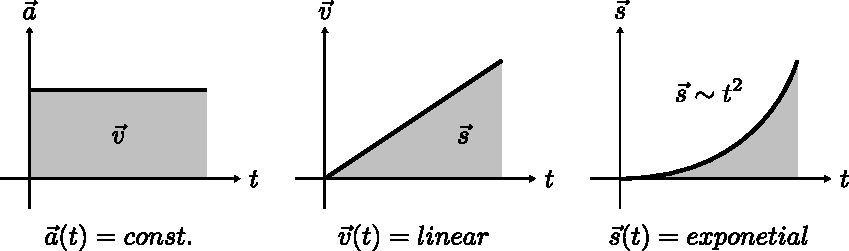
\includegraphics[scale=0.7]{bewegung.pdf}
	\caption{Gleichmässig beschleunigte Translation.}
	\label{fig:bewegung}
\end{figure}

\noindent
Mit den in der Grafik \ref{fig:bewegung} gezeigten Zusammenhängen lassen
sich Geschwindigkeit $\vec{v}$ und Weg $\vec{s}$ wie folgt beschreiben.
\[ \boxed{\begin{array}{r l} 
	\vec{a}(t) 	&= \displaystyle
		\vec{a} \\
	& \\
	\vec{v}(t)	&= \displaystyle 
		\vec{v}_0+\vec{a}\cdot t \\
	& \\
	\vec{s}(t) 	&= \displaystyle 
		\vec{s}_0+\vec{v}_0\cdot t+\frac{1}{2}\cdot\vec{a}\cdot t^2
\end{array}}\]
Bei einer solchen Bewegung mit konstanter Beschleunigung $\vec{a}$ gelten
insbesondere auch die folgenden Vereinfachungen.
\[ \boxed{\begin{array}{r l}
	\Delta \vec{s}	&= \displaystyle
		\vec{s}-\vec{s}_0 = \displaystyle
		\vec{v}_0\cdot t+\frac{1}{2}\cdot \vec{a}\cdot t^2 \\
	& \\
	\vec{v}^2 	&= \displaystyle
		\vec{v}_{0}^{2}+2\vec{a} \cdot \Delta \vec{s} \\
	& \\
	\vec{v}_{av} &= \displaystyle
		\frac{1}{2} \left( \vec{v}_0 + \vec{v} \right) \\
	& \\
	\vec{a} 	&= \displaystyle
		\frac{\vec{v}(t)^2-\vec{v}_0^2}{2\cdot\Delta \vec{s}} 
\end{array}}\]
Mit den obigen Vereinfachungen lassen sich nun die Formeln für 
$\vec{a}$, $\vec{v}$, $\vec{s}$ und $t$ durch je drei
Kombinationen formulieren (Winz'sche Tabelle).
\[ \boxed{\begin{array}{c c c c c c c}
	\vec{s}	
		&=& \displaystyle 
			\frac{1}{2} \cdot \vec{v} \cdot t
		&=& \displaystyle 
			\frac{1}{2} \cdot \frac{\vec{v}^2}{\vec{a}}
		&=& \displaystyle 
			\frac{1}{2} \cdot \vec{a} \cdot t^2 \\
	& & & & & & \\
	\vec{v} 
		&=& \displaystyle 
			\frac{1}{2} \cdot \frac{\vec{s}}{t}
		&=& \displaystyle 
			\sqrt{2 \cdot \vec{a} \cdot \vec{s}}
		&=& \displaystyle 
			\vec{a} \cdot t \\
	& & & & & & \\
	\vec{a}
		&=& \displaystyle 
			\frac{\vec{v}}{t} 
		&=& \displaystyle 
			\frac{1}{2} \cdot \frac{\vec{v}^2}{\vec{s}}
		&=& \displaystyle 
			2 \cdot \frac{\vec{s}}{t^2} \\
	& & & & & & \\
	t 	
		&=& \displaystyle 
			\frac{\vec{v}}{\vec{a}}
		&=& \displaystyle 
			\sqrt{\frac{2 \cdot \vec{s}}{\vec{a}}}
		&=& \displaystyle 
			2 \cdot \frac{\vec{s}}{\vec{v}}
\end{array}}\]

\section{Bewegung im Raum}
Da die Grössen der Bewegung vektoriell sind, können diese auch 
komponentenweise betrachtet werden.
\[ \boxed{\begin{array}{r l}
	\vec{\Delta r} &
		= \vec{r}_2-\vec{r}_1
		= (x_2-x_1,y_2-y_1,z_2-z_1) \\
	& \\
	v \rightarrow \vec{v} &
		= \lim\limits_{\Delta t \rightarrow 0}
			{\frac{\Delta \vec{r}}{\Delta t}}
		= \frac{d\vec{r}}{dt}
		= \left(\frac{dx}{dt},\frac{dy}{dt},\frac{dz}{dt}\right) \\
	& \\
	a \rightarrow \vec{a} &
		= \lim\limits_{\Delta t \rightarrow 0}
			{\frac{\Delta \vec{v}}{\Delta t}}
		= \frac{d\vec{v}}{dt}
		= \frac{d^2\vec{r}}{dt^2}
\end{array}}\]
		
\section{Bahnkurve}

\begin{figure}[h!]
	\centering
	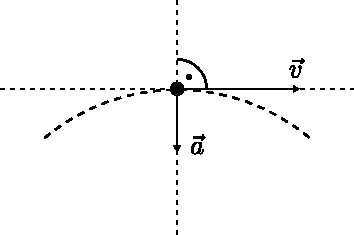
\includegraphics[scale=0.8]{bahnkurve.pdf}
	\caption{Bahnkurve mit Tangente und Normale dazu.}
	\label{fig:bahnkurve}
\end{figure}

\noindent
Betrachtet man die Grössen der Bewegung als Vektoren, so können diese 
in ihre jeweiligen Komponenten in $x,y,z$ zerlegt werden. Hierbei gilt 
insbesondere für die Geschwindigkeit $\vec{v}$ und die Beschleunigung
$\vec{a}$, dass diese entlang einer Bahnkurve stets normal zueinander 
sind oder anders formuliert:

\begin{itemize}
	\item Die Geschwindigkeit $\vec{v}$ liegt immer tangential an
		der Bahnkurve an.
	\item Gie Beschleunigung $\vec{a}$ zeigt immer nach innen, 
		d.h. normal zur Geschwindigkeit $\vec{v}$.
\end{itemize}

\section{Schiefer Wurf}
Der schiefe Wurf bezeichnet eine überlagerte Bewegung in mindestens zwei
Richtungen (z.B. $x$ und $y$). Diese Bewegung kann komponentenweise 
analysiert werden und per Superposition wieder zusammengesetzt werden.

\[\boxed{\begin{array}{r l  r l}
	& \vec{x}\text{-Komponente} & & \vec{y}\text{-Komponente} \\
	& & & \\
	\vec{a}_x 
		& = 0 
		& \qquad \vec{a}_y 
		& = -\vec{g} \\
	 & & &  \\
	\vec{v}_x 
		& = \vec{v}_0 \cdot cos(\alpha_0)
		& \vec{v}_y
		& = \vec{v}_0 \cdot sin(\alpha_0) -\vec{g} \cdot t \\
	 & & & \\
	\vec{s}_x
		& = \left( \vec{v}_0 \cdot cos(\alpha_0) \right) \cdot t
		& \vec{s}_y
		& = \left( \vec{v}_0 \cdot sin(\alpha_0) \right) \cdot t 
			- \frac{1}{2}\vec{g} \cdot t^2
\end{array}}\]

\noindent
Aus den obigen Zusammenhängen zum schiefen Wurf lässt sich eine 
Bahngleichung aufstellen, welche die Funktionen von $\vec{x}(t)$ und
$\vec{y}(t)$ kombiniert zu einer Funktion $\vec{y}(\vec{x})$.

\begin{figure}[h!]
	\centering
	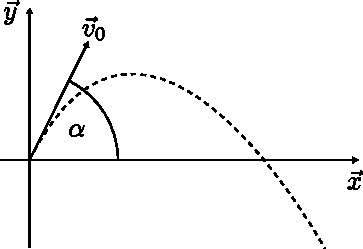
\includegraphics[scale=0.8]{wurf.pdf}
	\caption{Schiefer Wurf.}
	\label{fig:wurf}
\end{figure}

\[ \boxed{
	\vec{y} = \vec{x} \cdot tan(\alpha) 
		- \frac{\vec{g}}{2 \cdot \vec{v}_0^2 \cdot cos^2(\alpha)}
		\cdot \vec{x}^2
} \]

\noindent
Wichtig ist hierbei zu beachten, dass die passende Referenz für $\vec{y}$
gewählt wird, denn es gelten dann die folgenden Bedingungen.

\[ \boxed{\begin{array}{l l}
	\text{Landestelle tiefer als Abwurfstelle} & \Rightarrow y < 0 \\
	& \\
	\text{Landestelle gleich wie Abwurfstelle} & \Rightarrow y = 0 \\
	& \\
	\text{Landestelle höher als Abwurfstelle} & \Rightarrow y > 0 
\end{array}} \]


\section{Schräge Zerlegung}
Die Komponentenzerlegung eines Vektors kann beliebig erfolgen. 
D.h. die Zerlegung muss nicht zwingend in $x,y$ oder $z$ erfolgen,
sondern beliebig im Raum. Bei einigen Bewegungen ist dies von Vorteil,
etwa beim waagrechten Wurf (Spezialfall des schiefen Wurfs).

\begin{figure}[h!]
	\centering
	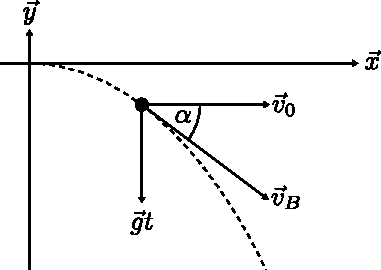
\includegraphics[scale=0.8]{wurf2.pdf}
	\caption{Schräge Komponentenzerlegung am waagrechten Wurf.}
	\label{fig:wurf2}
\end{figure}

\noindent
Mit dieser Zerlegung können die folgenden Zusammenhänge formuliert werden.
\[ \boxed{\begin{array}{r l}
	\vec{s} &
		= \vec{v}_0 \cdot t
		= \vec{v}_0 \cdot \sqrt{\frac{2 \cdot \vec{y}}{\vec{g}}} \\
	& \\
	\vec{y} &
		= \frac{1}{2} \cdot \vec{g} \cdot t^2 \\
	& \\
	\vec{v}_B &
		= \vec{v}_0 + \vec{g} \cdot t 
\end{array}}\]

